\section{Ruta 1: Universidad de Tokyo}

Ejecutamos la herramienta usando la dirección \texttt{www.u-tokyo.ac.jp}, con ráfagas de 100 paquetes y TTL máximo igual a 30. Los resultados obtenidos se muestran en las figuras \ref{tabla1} y \ref{mapa1}. Las ubicaciones indicadas fueron obtenidas usando una página de geolocalización de IP \cite{ip2location}.

\subsection{Análisis de la ruta obtenida}
Observamos que la ruta parte de Buenoa Aires como corresponde. Luego de no obtener respuesta en varios saltos, encontramos una IP supuestamente localizada en Italia. En el salto siguiente la IP se encuentra en Brasil.

Esto nos hizo sospechar acerca de la correctitud de esta ruta, ya que existen caminos directos entre Argentina y Brasil; no hay necesidad de pasar por Italia. Esto se puede ver en un mapa de cables submarinos \cite{cables}.

Como vimos que varias páginas de geolocalización de IP daban resultados distintos para la misma IP, usando una página que da resultados de fuentes distintas \cite{iplocation} comparamos resultados para la IP \texttt{195.22.219.3}. Obtuvimos como resultado que casi todas las fuentes devuelven una ubicación en Italia, mientras que una devuelve la ciudad de Fortaleza, en Brasil. Observamos que el cable submarino Altantis-2 conecta entre otras ciudades Las Toninas con Fortaleza \cite{atlantis2}. Además, figura como uno de los dueños del cable la empresa Telecom Italia Sparkle, que figura como ISP en varias búsquedas que ubican esta IP en Italia. Por esto creemos que la verdadera ruta va directamente hacia Fortaleza usando el cable Atlantis-2, ya que los métodos de geolocalización de IPs no son muy confiables \cite{accuracy}, y podría ocurrir que la ubicación de una IP situada físicamente en Brasil pero vinculada a una ISP italiana sea medida incorrectamente.

Luego la ruta sigue por San Pablo, y luego salta hasta Nueva York. En este caso mirando el mapa \cite{cables} vemos que se usa el cable Seabras-1, que une estas dos ciudades \cite{seabras1}.

Siguiendo por Estados Unidos, la ruta pasa por Seattle y salta hasta Osaka, en Japón. Esto es posible si se usa el cable Pacific Crossing-1, que entre otras ciudades une Shima, Japón (cercana a Osaka) con la zona de Seattle \cite{pc1}.

Finalmente se llega al destino en Tokyo.

\subsection{Análisis de las predicciones de salto intercontinental}

En la tabla de la figura \ref{tabla1} vemos que la mayoría de los saltos son incorrectamente predichos. Sólo $\frac{5}{16}$ resultan correctos, en total. Observamos que todos las predicciones incorrectas son falsos positivos. Lo analizamos por partes:

Porcentaje de saltos que no responden: 30,43\%

Largo de la ruta de saltos que responden: 16 saltos 

Cantidad de enlaces intercontinentales (separando América del Sur/Norte): 2

Cantidad de outliers: 14

Falsos positivos: 11

Falsos negativos: 0

\begin{figure}[H]
\centering
\begin{tabular}{l | l | l | l | c | c}
Hop & RTT & IP & Ubicación & Predicción de SI & ¿correcto?\\
\hline
1 & 0.0200 & 192.168.0.1 & Buenos Aires, Argentina & true & \xmark\\
2 & null & null & null & null\\
3 & null & null & null & null\\
4 & null & null & null & null\\
5 & null & null & null & null\\
6 & 0.0742 & \texttt{200.89.161.85} & Buenos Aires, Argentina & false & \cmark\\
7 & 0.0369 & \texttt{200.89.165.197} & Buenos Aires, Argentina & true & \xmark\\
8 & 0.0434 & \texttt{200.89.165.222} & Buenos Aires, Argentina & true & \xmark\\
9 & 0.0219 & \texttt{185.70.203.32} & Buenos Aires, Argentina & true & \xmark\\
10 & 0.0604 & \texttt{195.22.219.3} & Italia/Fortaleza, Brasil & true & \xmark\\
11 & 0.1129 & \texttt{149.3.181.65} & San Pablo, Brasil & false & \cmark\\
12 & 0.1700 & \texttt{129.250.2.227} & Nueva York, EEUU & true & \cmark\\
13 & 0.2852 & \texttt{129.250.4.13} & Seattle, EEUU & true & \xmark\\
14 & 0.4943 & \texttt{129.250.2.54} & Seattle, EEUU & true & \xmark\\
15 & 0.4242 & \texttt{129.250.3.61} & Osaka, Japón & true & \cmark\\
16 & 0.9055 & \texttt{129.250.5.41} & Osaka, Japón & true & \xmark\\
17 & 0.6164 & \texttt{129.250.3.106} & Osaka, Japón & true & \xmark\\
18 & 0.3777 & \texttt{61.200.80.218} & Osaka, Japón & true & \xmark\\
19 & null & null & null & null\\
20 & null & null & null & null\\
21 & null & null & null & null\\
22 & 0.3522 & \texttt{154.34.240.254} & Tokyo, Japón & true & \xmark\\
23 & 0.4735 & \texttt{210.152.135.178} & Tokyo, Japón & true & \xmark\\
\end{tabular}
\caption{Tabla de resultados para la Universidad de Tokyo.}
\label{tabla1}
\end{figure}

\begin{figure}[H]
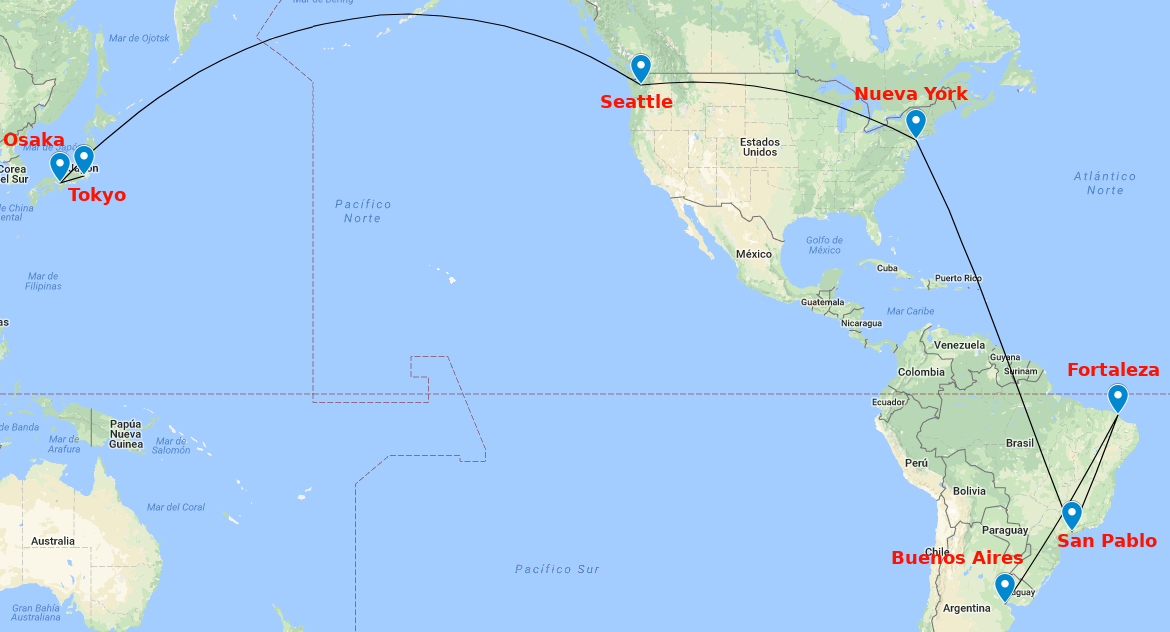
\includegraphics[width=\textwidth]{tokyo.png}
\caption{Mapa de resultados para la Universidad de Tokyo.}
\label{mapa1}
\end{figure}

\begin{figure}[H]
\centering
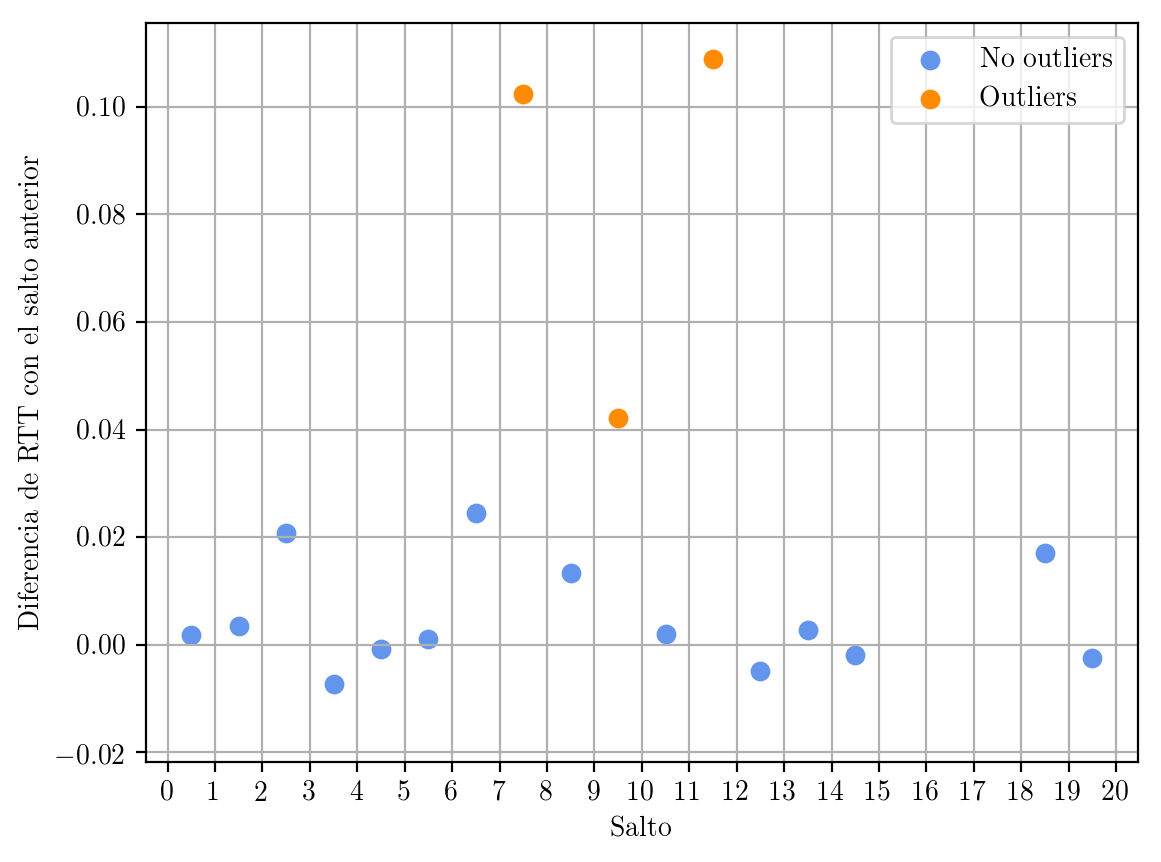
\includegraphics[width=0.6\textwidth]{tokyo1.png}
\caption{Gráfico de diferencias de RTT en función de cada salto.}
\label{diff1}
\end{figure}

\begin{figure}[H]
\centering
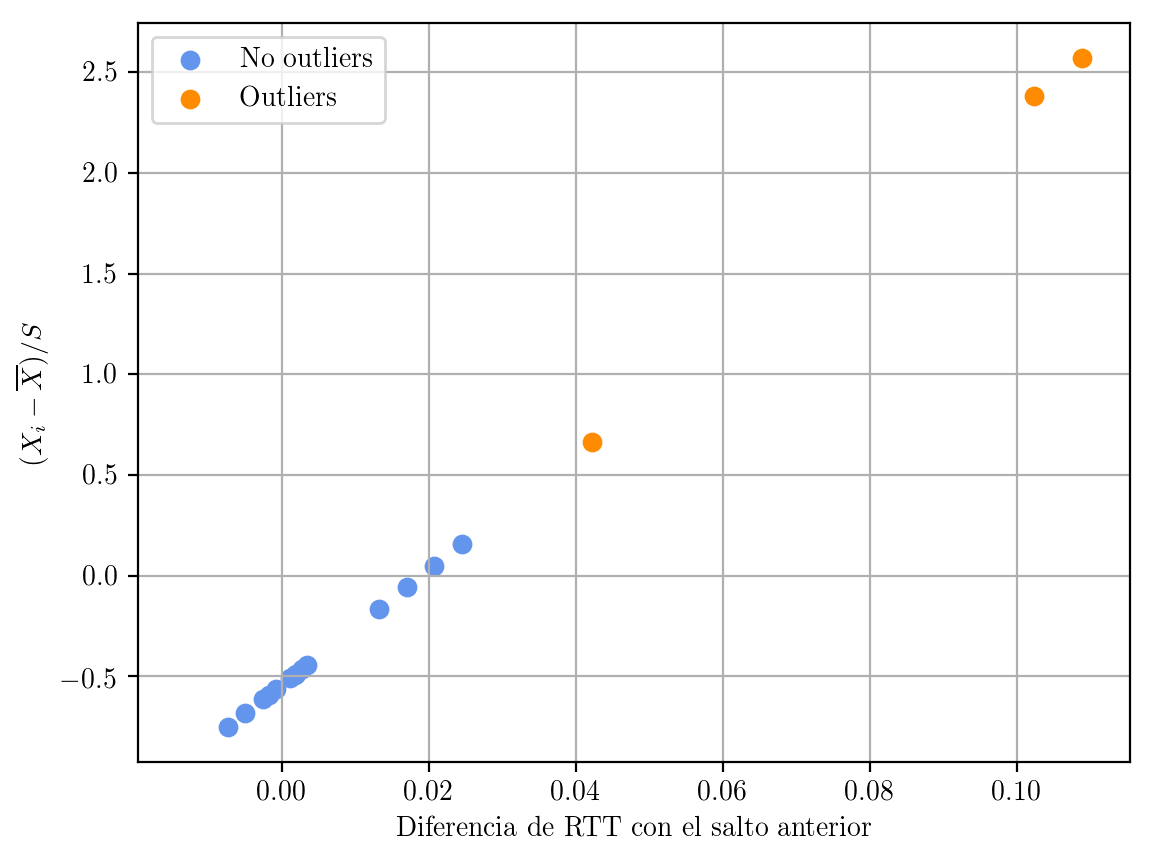
\includegraphics[width=0.6\textwidth]{tokyo2.png}
\caption{Gráfico de $\frac{X_i - \bar{X}}{S}$ en función de las diferencias de RTT.}
\label{sdev1}
\end{figure}